\subsection{Activation functions}
Rumelhart revised the structure of MLP to make backprop function properly: they replaced out the step function for the logistic function, better known as the \textit{sigmoid function}. This was crucial because there is no gradient to work with in the step function because the gradient descent cannot move on a flat surface, allowing it to advance somewhat at each step. The step function only contains flat segments. In actuality, aside from the sigmoid function, the backpropagation algorithm performs well with a wide variety of alternative activation functions. Here are two other popular choices. In the Figure \ref{fig:Activation Functions}, it's possible to see how they work.
\begin{itemize}
    \item \textit{The hyperbolic tangent function:} $tanh(z) = 2\sigma(2z) - 1$

    This activation function is S-shaped, continuous, and differentiable just like the sigmoid function, however its output value spans from -1 to 1, as opposed to 0 to 1, in the case of the sigmoid function. Because of this range, the output of each layer is more or less centered at zero at the start of training.

    \item \textit{The rectified linear unit function:} $ReLU(z) = max(0, z)$

    Although continuous, the ReLU function is unfortunately not differentiable at $z = 0$ and its derivative is $0$ for $z < 0$. But since it performs so well in practice and offers the benefit of being quick to compute, it has taken over as the standard. Since biological neurons appear to implement an activation function that is roughly sigmoid (S-shaped), researchers have focused on sigmoid functions for a very long time. ReLU, however, really performs better in ANNs in general. The biological analogy may have been misleading in this instance.
\end{itemize}
Why do we need activation functions? All you get when you combine many linear transformations is another linear transformation. Therefore, if there is no nonlinearity between the levels, even a deep stack of layers is equivalent to one layer, making it impossible to handle extremely complicated issues.
\begin{figure}
    \centering
    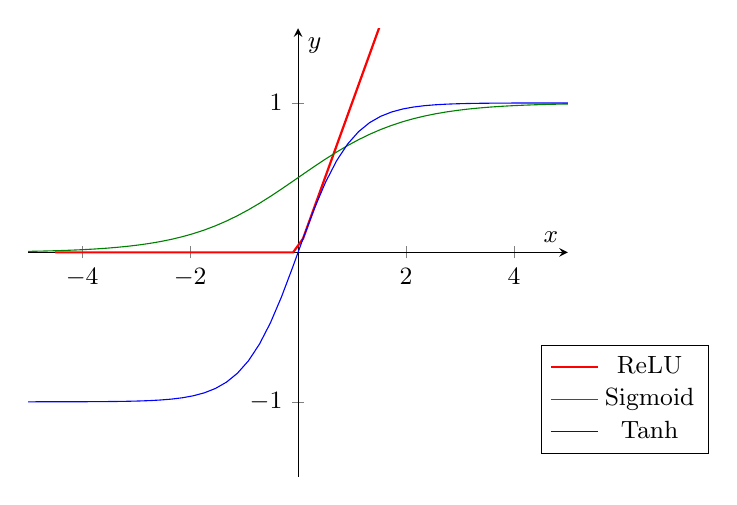
\begin{tikzpicture}
        \begin{axis}[
            axis lines = middle,
            xlabel = \(x\),
            ylabel = \(y\),
            xmin=-5.0,
            xmax=5.0,
            ymin=-1.5, 
            ymax=1.5,
            legend entries={ReLU,tanh,sigmoid},
            legend style={at={(0.95,0.05)},anchor=south west},
            %legend image post style={sharp plot,draw=red},
            cycle list name=color list,
            font=\small,
        ]
        % ReLU
        \addplot[color = red, thick, domain=-4.5:4.5, samples = 50] {max(0,x)};
        \addlegendentry{ReLU}
        % Sigmoid
        \addplot[color = green!50!black, samples=50] {1/(1+exp(-x))};
        \addlegendentry{Sigmoid}
    
        % tanh
        \addplot[color = blue, samples=50] {tanh(x)};
        \addlegendentry{Tanh}
        \end{axis}
    \end{tikzpicture}
    \caption{Activation Functions (ReLU, Sigmoid, Tanh) - Activation functions determine the output of a neuron in a neural network, and ReLU, Sigmoid, and Tanh are some commonly used activation functions that enable non-linear transformations of input data.}
    \label{fig:Activation Functions}
\end{figure}
